\chapter{UML}
\label{chap:uml}
\textbf{UML (Unified Modeling Language)} è un linguaggio di modellazione standard utilizzato per analizzare, progettare e documentare sistemi software. UML permette di rappresentare graficamente la struttura e il comportamento del sistema, comunicare in modo chiaro tra tutte le figure partecipanti allo sviluppo e documentare le decisioni di analisi e design in modo coerente. \\
UML mette a disposizione 14 tipi di diagrammi per la modellizazione del sistema e descrizione del suo comportamento.
\begin{figure}[h]
    \centering
    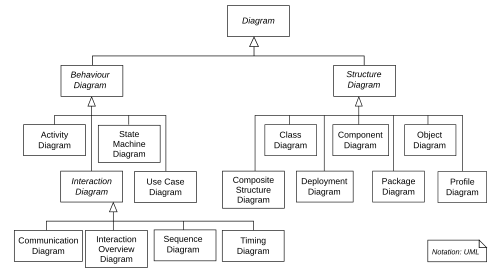
\includegraphics[width=1\linewidth]{IDSTEORIA/Immagini/UML/UMLDiagrammi.png}
    \caption{Organizzazione dei diagrammi in UML.}
\end{figure}

\section{Diagrammi Comportamentali}
\subsection{Use Case Diagram}
\label{diagram:usecase}
I meccanismi base di individuazione e definizione dei casi d'uso son già stati esplicati nella \hyperref[concept:casi-duso]{sezione dedicatali}. In questa sezione pertanto ci si limiterà a presentare il diagramma dei casi d'uso, tenendo conto della sua notazione grafica e di eventuali meccanismi avanzati legati all'uso degli UC. \\
I diagrammi dei \hyperref[concept:casi-duso]{casi d'uso} (o \textbf{Use Cases Diagram}) sono uno strumento dell'UML utilizzato per rappresentare tutti i casi d'uso presenti nel sistema e gli attori che li attivano. \\
L'obiettivo è mostrare quali sono le funzionalità del sistema, senza entrare nei dettagli implementativi del come vengono ottenute. Ogni \hyperref[concept:casi-duso]{UC} descrive un'interazione significativa tra un attore e il sistema stesso, finalizzata a raggiungere un certo obiettivo. \\
Un diagramma dei casi d'uso è quindi uno dei primi diagrammi da sviluppare in sviluppo ed è composto da:
\begin{itemize}
    \item \textbf{Attori} che rappresentano chi interagisce con il sistema attivando i casi d'uso. Sono rappresentati da uno stickman.
    \item \textbf{Casi d'uso} che rappresentano le funzionalità fornite dal sistema, rappresentati da un ovale.
    \item \textbf{Relazioni} tra attori e casi d'uso (attivazione) e tra casi d'uso stessi (inclusione, estensione, generalizzazione). Rappresentati attraverso delle linee.
    \item \textbf{Dominio} limiti del sistema o componente a cui sono associati determinati casi d'uso. Rappresentati da rettangoli.
\end{itemize}
\begin{figure}[h]
    \centering
    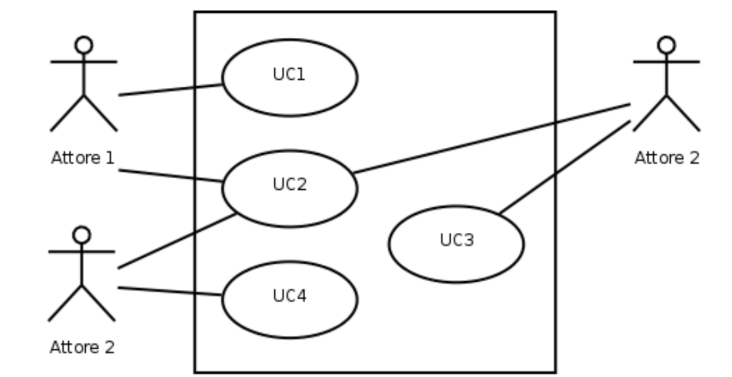
\includegraphics[width=0.80\linewidth]{IDSTEORIA/Immagini/UML/UC_base.png}
    \caption{Rappresentazione base di un diagramma dei casi d'uso.}
    \label{fig:uc_base}
\end{figure}
\subsubsection{Meccanismi avanzati}
UML mette a disposizione alcuni meccanismi avanzati per la rappresentazione degli UC. \\
Nello specifico:
\begin{itemize}
    \item \textbf{Generalizzazione degli attori}, attori con comportamenti o UC attivabili in comune possono essere generalizzati da un unico attore.
    \item \textbf{Generalizzazione tra casi d'uso}, i casi d'uso possono ereditare, aggiungere o ridefinire comportamenti da altri UC.
    \item \textbf{Inclusione $<<$include$>>$}, riutilizzare comportamenti comuni tra casi d'uso.
    \item \textbf{Estensione $<<$extend$>>$}, permette di aggiungere funzionalità opzionali o condizionali.
\end{itemize}
\begin{figure}[h]
    \centering
    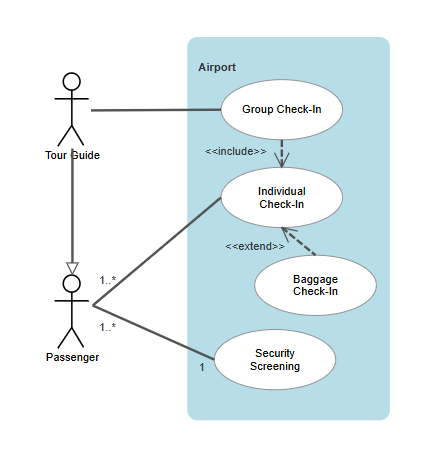
\includegraphics[width=0.7\linewidth]{IDSTEORIA/Immagini/UML/Esempio_UC_Diagram.png}
    \caption{Esempio di Use Cases Diagram che fa uso dei meccanismi avanzati.}
    \label{fig:UC_avanzato}
\end{figure}
Ad esempio, nella Figure \ref{fig:UC_avanzato}, l'attore Tour Guide è una composizione di attori Passenger. L'attore Tour Guide può inoltre attivare un solo caso d'uso: Group Check-in. Quest'ultimo caso d'uso include al suo interno il caso d'uso Individual Check-in, che a sua volta viene esteso da Baggage Check-in. 
\subsection{Sequence Diagram}
I \textbf{diagrammi di sequenza} (o Sequence Diagram) descrivono attraverso notazione grafica come gli oggetti interagiscono tra di loro per realizzare un certo comportamento. Sono composti da:
\begin{figure}[h]
    \centering
    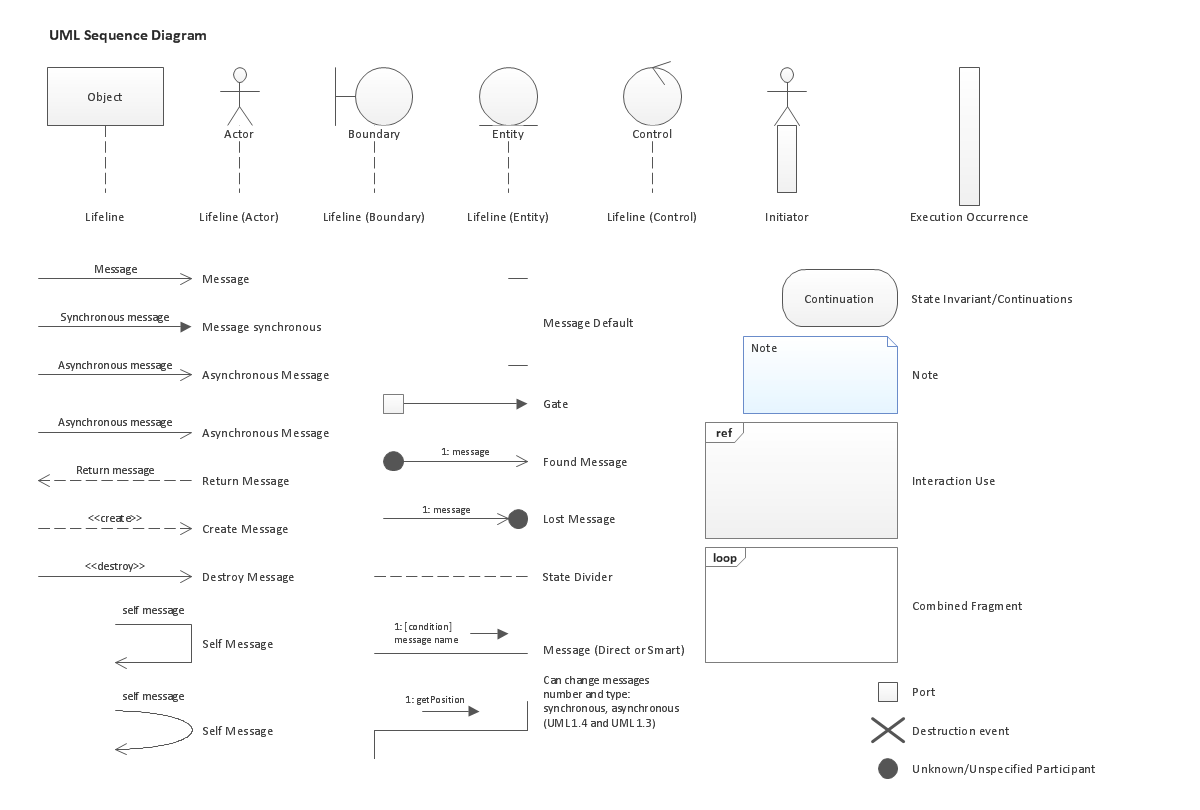
\includegraphics[width=1\linewidth]{IDSTEORIA/Immagini/UML/UMLSequenceDiagramElements.png}
    \caption{Notazione grafica dei vari elementi del Sequence Diagram.}
    \label{fig:seq_elements}
\end{figure}
\begin{itemize}
    \item \textbf{Linee di vita (o lifelines)}, oggetti o classi coinvolte nell'interazione, sono rappresentati da un rettangolo contenente le informazioni base (nome, tipo) e da una linea verticale rappresentante la durata dell'esistenza nel sistema.
    \item \textbf{Messaggi}, sono l'interazione tra due lifeline. Possono essere:
    \begin{itemize}
        \item Chiamate di operazione 
        \item Risposte
        \item Chiamate di creazione/distruzione
    \end{itemize}
\end{itemize}


Ulteriori approfondimenti sulle norme per realizzare i Sequence Diagram nell'\hyperref[appendix:sequence]{apposita appendice}.
\newpage
\section{Diagramma di Attività}
I \textbf{Diagrammi di Attività} (o \textbf{Activity Diagram}) servono a rappresentare graficamente lo scenario principale di un caso d'uso e le sue varianti, visualizzare la sequenza di azioni e le decisioni prese dagli attori ed individuare punti di parallelismo. \\
La loro semantica è basata sulle \hyperref[concept:petrinets]{Reti di Petri}, dove il flusso di controllo è rappresentato da token che si spostano lungo gli archi. 
\paragraph{Tipologie di nodi}
Gli elementi di un diagramma di attività sono:
\begin{itemize}
    \item \textbf{Nodi azione}, operazioni elementari
    \item \textbf{Nodi di controllo}, gestiscono il flusso dei token
    \item \textbf{Nodi oggetto}, rappresentano dei buffer di dati presenti nel flusso
    \item \textbf{Flussi di controllo}, gestiscono il flusso logico attraverso i token
    \item \textbf{Flussi di oggetti}, gestiscono il flusso di dati tra le varie azioni
\end{itemize}
\paragraph{Nodi principali} I principali nodi dell'Activity Diagram sono:
\begin{itemize}
    \item \textbf{start node}, definisce dove inizia il flusso
    \item \textbf{action node}, indica una specifica azione, quando l'azione è terminata viene rilasciato un token
    \item \textbf{final flow node}, nodo di terminazione per quel specifico flusso
    \item \textbf{final activity node}, nodo di terminazione per l'intera attività, in caso di parallelismo anche gli altri flussi vengono interrotti
    \item \textbf{decision node}, permette la creazione di sequenze alternative
    \item \textbf{merge node}, definisce dove la sequenza alternativa si riunisce a quella principale
    \item \textbf{fork}, divide il flusso in più sotto-flussi che avanzano in parallelo
    \item \textbf{join}, termina il parallelismo
\end{itemize}
\begin{figure}[h]
    \centering
    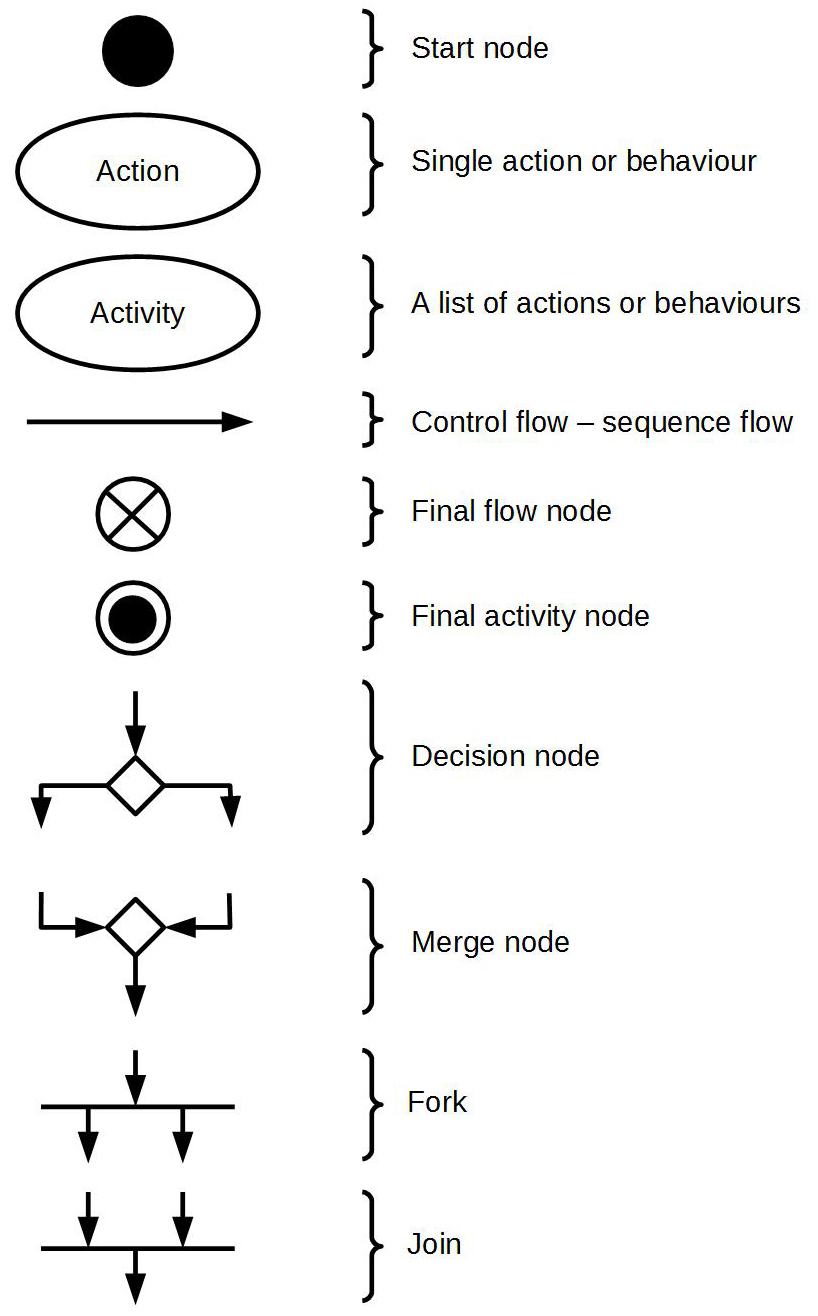
\includegraphics[width=0.75\linewidth]{IDSTEORIA/Immagini/UML/ActivityDiagram.png}
    \caption{Notazione grafica dei vari elementi di un Activity Diagram.}
\end{figure}